\documentclass{NRVposter}
\usepackage{graphicx}
\usepackage{hyperref}

\title{NRV Framework}
\author{T. Couppey, L. Regnacq, R. Giraud, O. Romain, Y. Bornat, F. Kolbl}
\institute{
    Laboratory ETIS - UMR CNRS 8051, ENSEA, CY - Cergy, France\\
    Laboratory IMS - UMR CNRS 5218, Bordeaux INP, U. Bordeaux - Talence, France}


\begin{document}
\maketitle

% Tip: for long titles, use \parbox{\linewidth}{text}

%\block{Abstract}{This is a description of the class to make posters according 
%to NRV's official template.}

\begin{columns}
\column{0.62}
\block{The NeuRon Virtualizer: a pythonic tool for simulating neural interfaces}{
    NRV is a pythonic framework to enable fast and user friendly simulations of the Peripheral Nervous System. Axons models are simulated with the NEURON software, and extracellular fields are computed either from analytic equations such as point source approximation or with a more detailed description of the nerve and electrode geometry and Finite Elements Method, either using COMSOL (additional commercial licence requiered) or the FENICS project. Stimulation waveform can be of random shapes, and any kinds of electrode can be combined to model complex stimulation strategies.

    NRV has been optimized for large population of axons, from generating correct population following a specific diameter probability, through automatic placement to computation and post-processing of the axons activity when a stimulus is applied. Parallel computation, interface with NEURON and COMSOL and FENICS is automatically handled by NRV. For a detailed description and full help on installation, basic usage and API documentation.
    \vspace{
        0.01\textheight
    }
    \begin{center}
        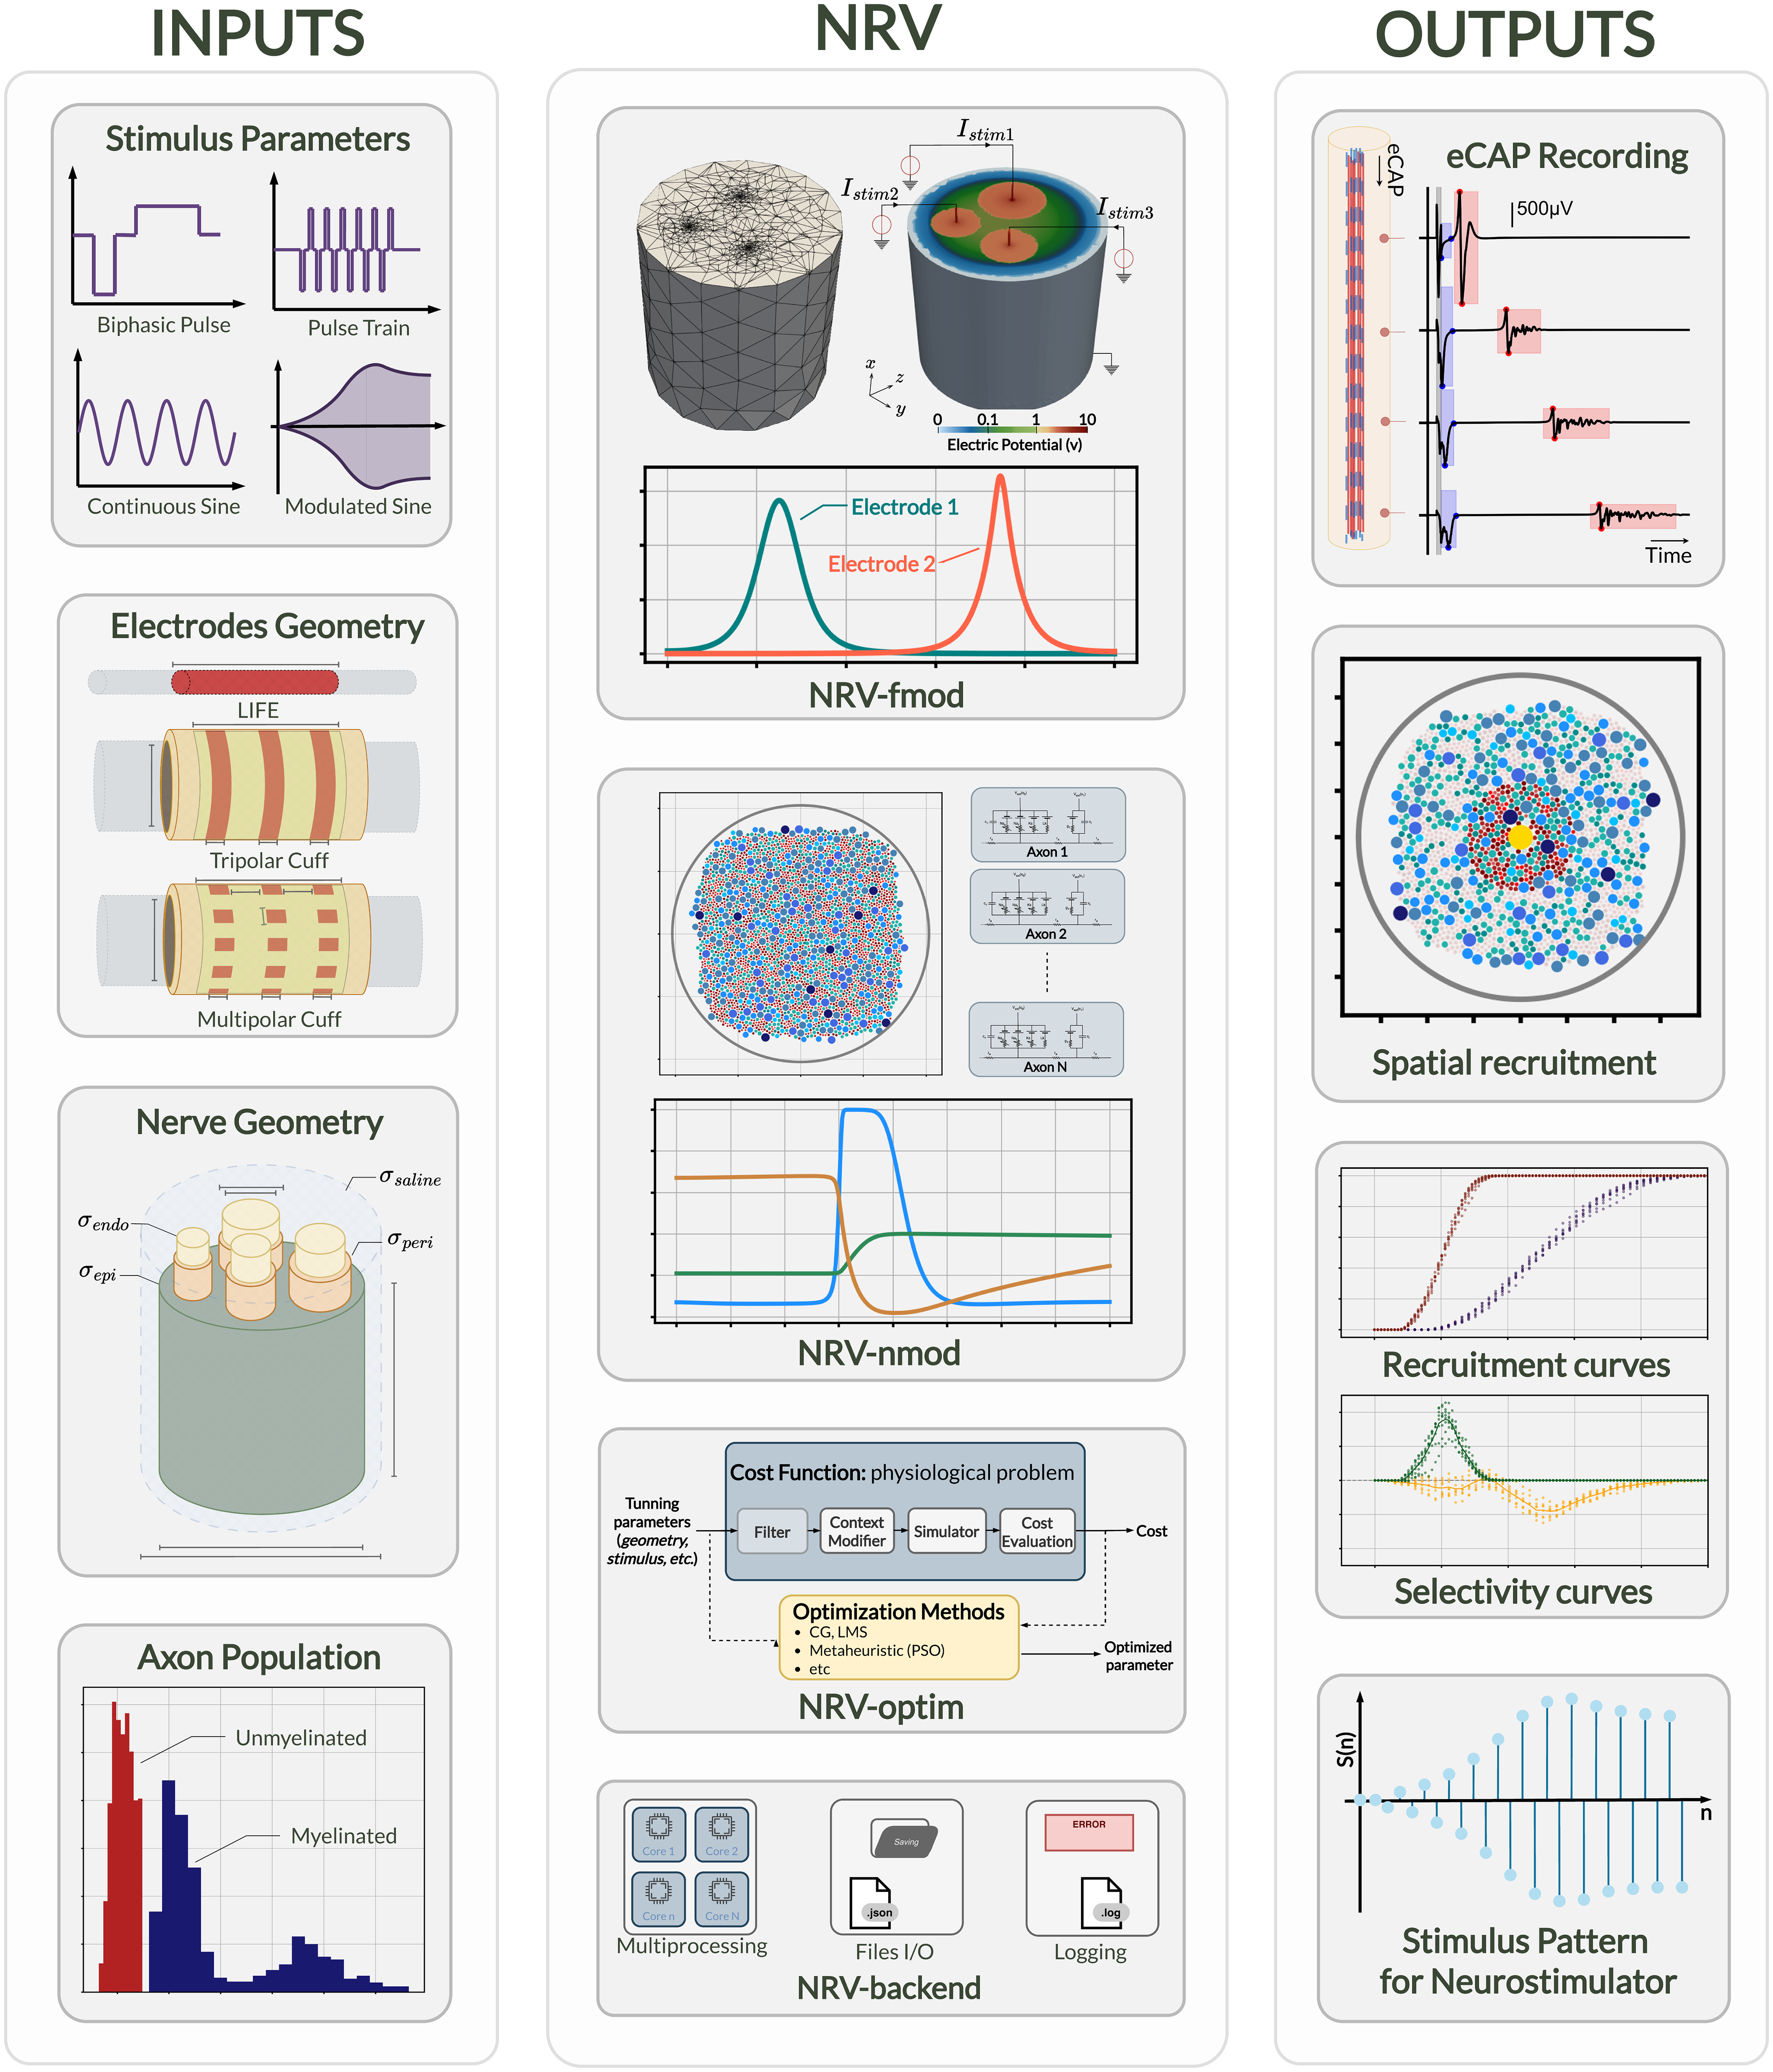
\includegraphics[width=0.45\columnwidth]{./images/overview.png}
    \end{center}

}


\block{Compilation \emph{will} fail on first attempt with hyperref}{
Due to a bug in \texttt{tikzposter}, compilation will always fail in the 
absence of an \texttt{.aux} file, i.e. when compiling for the first time, in 
case you included the \texttt{hyperref} package.
Just compile again and things will work fine.
This will eventually be corrected in \texttt{tikzposter}.
}

\column{0.38}
\block{Find us}
{
    \begin{itemize}
        \item \textbf{Access our website:} \\ \url{https://nrv-framework.org}\\
            \begin{center}
                
\includegraphics[width=0.08\columnwidth]{./images/qrcode_website.png}
            \end{center}
            and enter the forum for help (community page)
        \item  
\includegraphics[width=0.015\columnwidth]{./images/github_logo.png} \textbf{Access the source code:} \\ \url{https://github.com/nrv-framework/NRV}\\
            \begin{center}
                
\includegraphics[width=0.08\columnwidth]{./images/qrcode_github.png}
            \end{center}
        \item 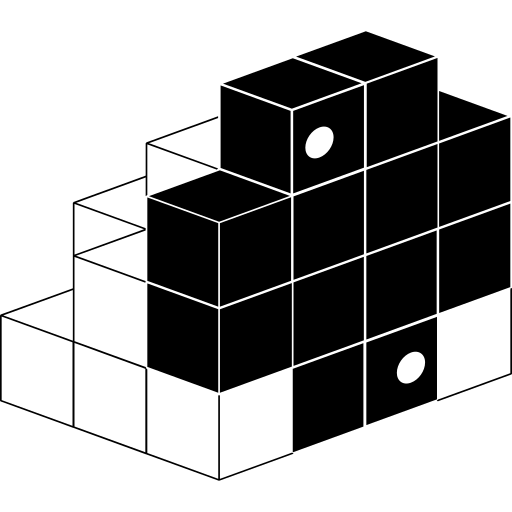
\includegraphics[width=0.015\columnwidth]{./images/pypi_logo.png} \textbf{Get the installer:} \\ \url{https://pypi.org/project/nrv-py/}\\
        \begin{center}
            
\includegraphics[width=0.08\columnwidth]{./images/qrcode_pypi.png}
        \end{center}
        \item 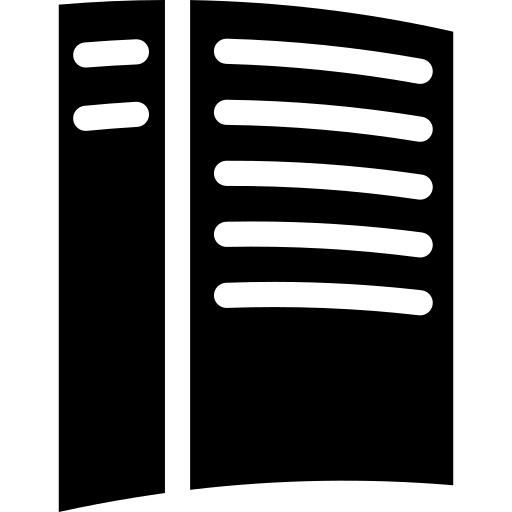
\includegraphics[width=0.015\columnwidth]{./images/rtd_logo.png} \textbf{Get the documentation:} \\ \url{https://nrv.readthedocs.io/en/latest/}\\
        \begin{center}
            
\includegraphics[width=0.08\columnwidth]{./images/qrcode_rtd.png}
        \end{center}
    \end{itemize}
    

    
}

\block{Help and contribute}{
to write!
}

\end{columns}


\end{document}

